
% 使用 XeLaTeX 编译
% 所需宏包：ctex、tikz、circuitikz、booktabs 等

\documentclass[UTF8,a4paper,12pt,fontset=none]{ctexart}

% ==================== 中文字体配置 ====================
\setCJKmainfont{STSong}
\setCJKsansfont{STHeiti}
\setCJKmonofont{STSong}
\setCJKfamilyfont{zhsong}{STSong}
\setCJKfamilyfont{zhhei}{STHeiti}
% ==================== 页面设置 ====================
\usepackage[
    left=2.25cm,
    right=2.25cm,
    top=2.15cm,
    bottom=2.2cm
]{geometry}

\usepackage{amsmath,amssymb}
\usepackage{booktabs,array,tabularx}
\usepackage{enumitem,float}
\usepackage{tikz,circuitikz}
\usetikzlibrary{arrows.meta,calc,positioning}
\usepackage{fancyhdr}

\pagestyle{fancy}
\fancyhf{}
\fancyhead[C]{\small 大 学 物 理 实 验 报 告}
\fancyfoot[C]{第\,\thepage\,页}
\renewcommand{\headrulewidth}{0.4pt}
\setlength{\headheight}{16pt}

\setlength{\parindent}{2em}
\setlength{\parskip}{0.3em}
\linespread{1.2}

\setlist[enumerate]{
    leftmargin=2.4em,
    itemsep=0.25em,
    topsep=0.25em
}

% ==================== 常用数学符号 ====================
\newcommand{\ddq}{\Delta q}
\newcommand{\Cb}{C_{\mathrm b}}
\newcommand{\Iplus}{I_{+}}
\newcommand{\Iminus}{I_{-}}
\newcommand{\Bres}{B_{\mathrm r}}

\begin{document}

% ==================== 标题 ====================

\begin{center}
{\LARGE\bfseries 磁性材料磁滞回线测量实验报告}\\[0.6em]
{\large 大学物理实验}
\end{center}

\noindent
\textbf{实验名称：}铁磁材料的磁化曲线与磁滞回线\\
\textbf{姓名：}\underline{\hspace{4cm}}
\quad
\textbf{学号：}\underline{\hspace{4cm}}
\quad
\textbf{日期：}\underline{\hspace{2.8cm}}

% ==================== 一、实验目的 ====================

\section{实验目的}

\begin{enumerate}
    \item 测量反映软磁材料的 $H$--$B$ 特性的特征参数。
    \item 绘制饱和磁滞回线，并从图中标出矫顽力
    $H_{\mathrm c}$。
\end{enumerate}

% ==================== 二、实验原理 ====================

\section{实验原理}

磁性材料在被磁化时，其磁感应强度 $B$ 随磁场强度 $H$
变化，但是 $B$ 与 $H$ 之间的函数关系非常复杂，
具有以下特征。

一块从未被磁化的材料磁化时，当 $H$ 由 $0$ 开始
逐渐增加至某一最大值 $H_{\mathrm m}$，
$B$ 也由 $0$ 开始逐渐增加，
由此画出的 $B$--$H$ 曲线 $OA$ 称为
\textbf{起始磁化曲线}。

起始磁化曲线大致分成三个阶段：
第一阶段曲线平缓，第二阶段曲线很陡，
第三阶段曲线又变得很平缓。

最后 $B$ 趋于不变，这种现象称为\textbf{饱和}。
饱和时的磁感应强度称为\textbf{饱和磁感应强度}，
记作 $B_{\mathrm s}$。

磁化过程中材料内部发生的过程是不可逆的。
当磁场由饱和时的 $H_{\mathrm m}$ 减小至 $0$，
$B$ 并非沿原来的起始磁化曲线返回，
而是滞后于 $H$ 的变化，
沿 $A\to B_{\mathrm r}$ 变化。

当 $H=0$ 时，$B=B_{\mathrm r}$，
称为\textbf{剩余磁感应强度}。

要想使 $B$ 为 $0$，
就必须施加反向磁场 $H_{\mathrm c}$，
$H_{\mathrm c}$ 称为\textbf{矫顽力}。

继续增大反向磁场至 $-H_{\mathrm m}$，
磁感应强度变为 $-B_{\mathrm s}$。

磁场再由 $-H_{\mathrm m}$ 变为 $H_{\mathrm m}$，
曲线沿另一支返回，形成一条闭合曲线，
称为\textbf{磁滞回线}。

% ==================== TikZ 磁滞回线 ====================

\begin{figure}[H]
\centering

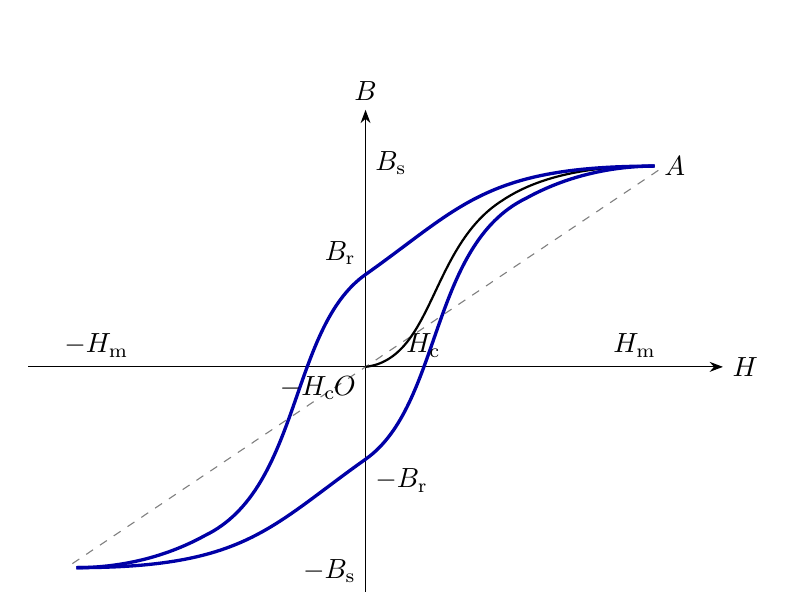
\begin{tikzpicture}[>=Stealth,scale=1.02]

% 坐标轴
\draw[->] (-4.2,0)--(4.45,0)
    node[right] {$H$};

\draw[->] (0,-3.0)--(0,3.2)
    node[above] {$B$};

% 辅助线
\draw[gray,dashed]
    (-3.65,-2.45)--(3.65,2.45);

% 起始磁化曲线
\draw[thick]
    (0,0)
    .. controls (0.85,0.1) and (0.8,1.5)
    .. (1.7,2.07)
    .. controls (2.25,2.44) and (3.0,2.5)
    .. (3.6,2.5);

% 磁滞回线上支
\draw[very thick,blue!65!black]
    (3.6,2.5)
    .. controls (1.5,2.5) and (1.2,2.0)
    .. (0,1.15)
    .. controls (-0.95,0.48) and (-0.8,-1.52)
    .. (-2,-2.1)
    .. controls (-2.6,-2.43) and (-3.2,-2.5)
    .. (-3.6,-2.5);

% 磁滞回线下支
\draw[very thick,blue!65!black]
    (-3.6,-2.5)
    .. controls (-1.5,-2.5) and (-1.2,-2.0)
    .. (0,-1.15)
    .. controls (0.95,-0.48) and (0.8,1.52)
    .. (2,2.1)
    .. controls (2.6,2.43) and (3.2,2.5)
    .. (3.6,2.5);

% 坐标标签
\node[below left] at (0,0) {$O$};
\node[right] at (3.6,2.5) {$A$};

\node[above left] at (0,1.15)
    {$B_{\mathrm r}$};

\node[below right] at (0,-1.15)
    {$-B_{\mathrm r}$};

\node[below] at (-0.72,0)
    {$-H_{\mathrm c}$};

\node[above] at (0.72,0)
    {$H_{\mathrm c}$};

\node[above] at (3.35,0)
    {$H_{\mathrm m}$};

\node[above] at (-3.35,0)
    {$-H_{\mathrm m}$};

\node[right] at (0,2.54)
    {$B_{\mathrm s}$};

\node[left] at (0,-2.54)
    {$-B_{\mathrm s}$};

\end{tikzpicture}

\caption{
$B$--$H$ 起始磁化曲线与磁滞回线示意图
（定性重绘）
}

\end{figure}

由法拉第电磁感应定律，
磁感应强度可通过冲击电流计的最大偏转测得：

\begin{equation}
\label{eq:core}
B=\frac{\Cb}{2N_2S}\,\alpha,
\qquad
\Cb=R C_{\mathrm b}^{\prime}.
\end{equation}

式中：

$\Cb$ 为冲击电流计常数；

$\alpha$ 为最大偏转读数；

$N_2$ 为次级线圈匝数；

$S$ 为次级线圈截面积。

对于磁感应强度的变化量，依据励磁电流是否反向，
计算中还会用到

\begin{equation}
\label{eq:delta}
\Delta B=\frac{\Cb}{N_2S}\,\ddq.
\end{equation}

% ==================== 三、实验仪器 ====================

\section{实验仪器}

冲击电流计、直流稳压电源、
0.5 级直流电流表、滑线变阻器、
换向开关、磁线环、线圈。

% ==================== 四、实验过程 ====================

\section{实验过程}

\subsection{实验步骤}

\begin{enumerate}

\item 用切纸打磨去除磁线环内的漆包线接头，
按实验电路连接线路。

\item 调整励磁电路的电源输出，
使最大励磁电流达到 $350\,\mathrm{mA}$。

\item 开始进行磁滞回线特征参数的测量。

\end{enumerate}

% ==================== Circuitikz 电路图 ====================

\begin{figure}[H]
\centering

\begin{circuitikz}[
    american currents,
    scale=0.91,
    transform shape
]

% 初级励磁回路
\draw
(0,0)
to[battery1,l_={直流电源}] (0,3.2)
to[spst,l={$K_2$}] (2,3.2)
to[ammeter,l={$I$}] (4,3.2)
to[vR,l={$R_1$}] (6,3.2)
to[L,l={$N_1$}] (6,0)
-- (0,0);

% 次级测量回路
\draw
(8,0)
to[L,l_={$N_2$}] (8,3.2)
to[spst,l={$K_3$}] (10,3.2)
to[R,l={$R$}] (12,3.2)
to[rmeterwa,l={$G$}] (12,0)
-- (8,0);

% 磁芯耦合关系
\draw[dashed,thick]
(6.6,0.45)--(7.35,0.45)
(6.6,2.7)--(7.35,2.7);

\node[align=center,font=\small]
at (7,1.5) {磁\!芯\\耦\!合};

\node[font=\small,align=center]
at (3,-0.65)
{励磁回路（换向操作由实际换向开关完成）};

\node[font=\small]
at (10,-0.65)
{冲击电流计回路};

\end{circuitikz}

\caption{
磁滞回线测量电路原理示意图
（按原图功能简化重绘）
}

\end{figure}

\subsection{操作要点：测量饱和磁滞回线}

\begin{enumerate}

\item 测量 $A$ 点时，将励磁电流按

\[
\Iminus\to\Iplus\to\Iminus
\]

改变，取平均读数 $\alpha$，
计算 $B_A(=B_{\mathrm s})$。

\item 励磁电流停留在 $A$ 点：

\[
I^{+}=350\,\mathrm{mA}.
\]

\item 测量 $B_{\mathrm r}$ 和 $B_{\mathrm r}'$。

励磁电流依次为

\[
\Iplus\to0
\xrightarrow{K_1\text{ 断开后接上}}
\Iminus
\xrightarrow{K_1\text{ 断开后接上}}
0\to\Iplus.
\]

磁化状态沿

\[
A\to r\to A'\to r'\to A
\]

变化。

测量各段的冲击电流计偏转，
求其平均值并计算剩磁。

\item 借助剩磁测量 $C_1$--$C_4$ 点的 $B$ 值。

使磁化状态回到 $A$ 点：

\[
I=350\,\mathrm{mA}.
\]

逐渐减小励磁电流，
使磁化状态移到 $C_1$ 点附近：

\[
I^{+}=200\,\mathrm{mA}.
\]

然后依次按表格记录各次偏转，
计算各点磁感应强度。

\end{enumerate}

% ==================== 测量安排 ====================

\begin{table}[H]
\centering
\small

\caption{磁滞回线特征点测量安排（据手稿整理）}

\begin{tabularx}{\linewidth}{
>{\raggedright\arraybackslash}p{2.4cm}
*{4}{>{\centering\arraybackslash}X}
}

\toprule
励磁电流
& $\Iplus\to0$
& $0\to\Iminus$
& $\Iminus\to0$
& $0\to\Iplus$
\\
\midrule

磁化状态
& $C_1\to r$
& $r\to C_2$
& $C_3\to r'$
& $r'\to C_4$
\\

读数
& $\Delta q_{C_1}$
& $\Delta q_{C_2}$
& $\Delta q_{C_3}$
& $\Delta q_{C_4}$
\\

\bottomrule

\end{tabularx}
\end{table}

% ==================== 五、实验结果 ====================

\section{实验结果与分析}

取实验公式

\begin{equation}
B=\frac{\Cb}{N_2S}\,Q.
\end{equation}

已知

\begin{align*}
\Cb &=1.034\times10^{-4}\ \mathrm{H\cdot A/C},\\
N_2 &=12,\\
S &=75.925\ \mathrm{mm^2}.
\end{align*}

其中按原报告保留符号 $Q$ 表示所记录的偏转读数。

以下数值统一采用

\[
S=75.925\times10^{-6}\,\mathrm{m^2}.
\]

% ==================== A、A' ====================

\subsection{计算 $A$ 与 $A'$ 点的 $B$}

\begin{table}[H]
\centering

\caption{饱和状态测量数据}

\begin{tabular}{lcc}
\toprule

励磁电流变化
& $\Iminus\to\Iplus$
& $\Iplus\to\Iminus$
\\
\midrule

磁化状态
& $A\to A'$
& $A'\to A$
\\

冲击电流计读数
& 6.73
& 6.42
\\

\bottomrule
\end{tabular}
\end{table}

计算平均值：

\begin{align*}
\overline{\Delta q}
&=\frac{6.73+6.42}{2}\\
&\approx6.58.
\end{align*}

计算饱和磁感应强度：

\begin{align*}
B_A
&=\frac12\frac{\Cb}{N_2S}
\,\overline{\Delta q}\\
&=\frac12
\times
\frac{1.034\times10^{-4}}
{12\times75.925\times10^{-6}}
\times6.58\ \mathrm T\\
&\approx0.373\ \mathrm T.
\end{align*}

因此

\[
\boxed{B_A\approx0.373\ \mathrm T}
\]

\[
\boxed{B_{A'}=-B_A\approx-0.373\ \mathrm T}
\]

% ==================== 剩磁 ====================

\subsection{计算 $r$ 与 $r'$ 点的 $B$}

\begin{table}[H]
\centering

\caption{剩磁及相关状态变化的偏转读数}

\begin{tabular}{lcccc}
\toprule

励磁电流
& $\Iplus\to0$
& $0\to\Iminus$
& $\Iminus\to0$
& $0\to\Iplus$
\\
\midrule

磁化状态
& $A\to r$
& $r\to A'$
& $A'\to r'$
& $r'\to A$
\\

读数
& 2.46
& 3.97
& 2.51
& 3.94
\\

\bottomrule
\end{tabular}
\end{table}

\noindent
\textbf{（1）$A\to r$：}

\begin{align*}
\Delta B_{A\to r}
&=\frac{\Cb}{N_2S}\times2.46\\
&\approx0.279\ \mathrm T.
\end{align*}

\begin{align*}
B_{\mathrm r}
&=B_{\mathrm s}-\Delta B_{A\to r}\\
&\approx0.373-0.279\\
&=0.094\ \mathrm T.
\end{align*}

\[
\boxed{B_{\mathrm r}\approx0.094\ \mathrm T}
\]

\noindent
\textbf{（2）$A'\to r'$：}

\begin{align*}
\Delta B_{A'\to r'}
&=\frac{\Cb}{N_2S}\times2.51\\
&\approx0.284\ \mathrm T.
\end{align*}

\begin{align*}
B_{\mathrm r}'
&=-\left(
B_{\mathrm s}-\Delta B_{A'\to r'}
\right)\\
&\approx-(0.373-0.284)\\
&=-0.089\ \mathrm T.
\end{align*}

\[
\boxed{B_{\mathrm r}'\approx-0.089\ \mathrm T}
\]

原手稿记录末项约为 $-0.088\,\mathrm T$；
本处按所列读数和系数直接计算，
差异属于中间数值取舍问题。

后续为与手稿所列结果对照，
相关点仍使用其

\[
|B_{\mathrm r}'|=0.088\,\mathrm T.
\]

% ==================== C1-C4 ====================

\subsection{计算 $C_1,C_2,C_3,C_4$ 处的 $B$}

\begin{table}[H]
\centering

\caption{磁滞回线上四个特征点的数据}

\begin{tabular}{lcccc}
\toprule

励磁电流
& $\Iplus\to0$
& $0\to\Iminus$
& $\Iminus\to0$
& $0\to\Iplus$
\\
\midrule

磁化状态
& $C_1\to r$
& $r\to C_2$
& $C_3\to r'$
& $r'\to C_4$
\\

读数
& 1.96
& 3.71
& 2.20
& 3.20
\\

\bottomrule
\end{tabular}
\end{table}

% ==================== C1 ====================

\noindent
\textbf{（1）$C_1\to r$：}

\begin{align*}
\Delta B_{C_1\to r}
&=\frac{1.034\times10^{-4}}
{12\times75.925\times10^{-6}}
\times1.96\\
&\approx0.222\ \mathrm T.
\end{align*}

\begin{align*}
B_{C_1}
&=\Delta B_{C_1\to r}+B_{\mathrm r}\\
&\approx0.222+0.094\\
&=0.316\ \mathrm T.
\end{align*}

% ==================== C2 ====================

\noindent
\textbf{（2）$r\to C_2$：}

\begin{align*}
\Delta B_{r\to C_2}
&=\frac{1.034\times10^{-4}}
{12\times75.925\times10^{-6}}
\times3.71\\
&\approx0.421\ \mathrm T.
\end{align*}

\begin{align*}
B_{C_2}
&=-\bigl(
\Delta B_{r\to C_2}-B_{\mathrm r}
\bigr)\\
&\approx-(0.421-0.094)\\
&=-0.327\ \mathrm T.
\end{align*}

% ==================== C3 ====================

\noindent
\textbf{（3）$C_3\to r'$：}

\begin{align*}
\Delta B_{C_3\to r'}
&=\frac{1.034\times10^{-4}}
{12\times75.925\times10^{-6}}
\times2.20\\
&\approx0.250\ \mathrm T.
\end{align*}

\begin{align*}
B_{C_3}
&=-\left(
\Delta B_{C_3\to r'}+|B_{\mathrm r}'|
\right)\\
&\approx-(0.250+0.088)\\
&=-0.338\ \mathrm T.
\end{align*}

% ==================== C4 ====================

\noindent
\textbf{（4）$r'\to C_4$：}

\begin{align*}
\Delta B_{r'\to C_4}
&=\frac{1.034\times10^{-4}}
{12\times75.925\times10^{-6}}
\times3.20\\
&\approx0.363\ \mathrm T.
\end{align*}

\begin{align*}
B_{C_4}
&=\Delta B_{r'\to C_4}-|B_{\mathrm r}'|\\
&\approx0.363-0.088\\
&=0.275\ \mathrm T.
\end{align*}

% ==================== 数据汇总 ====================

\subsection{实验结果汇总}

\begin{table}[H]
\centering

\caption{磁感应强度特征值（依据手稿计算结果）}

\begin{tabular}{ccccccccc}
\toprule

测量点
& $A$
& $A'$
& $r$
& $r'$
& $C_1$
& $C_2$
& $C_3$
& $C_4$
\\
\midrule

$B/\mathrm T$
& 0.373
& $-0.373$
& 0.094
& $-0.088$
& 0.317
& $-0.327$
& $-0.337$
& 0.275
\\

\bottomrule
\end{tabular}
\end{table}

% ==================== 绘制磁滞回线 ====================

\subsection{磁滞回线的绘制与矫顽力标注}

根据实验测得的特征点，
作 $H$--$B$ 曲线，
并在曲线与 $H$ 轴的交点处标出矫顽力
$H_{\mathrm c}$。

原始手稿未提供各点对应的完整磁场强度 $H$
测量值，因此下面仅给出\textbf{定性示意图}，
不将横轴视作实测刻度，
也不据此虚构 $H_{\mathrm c}$ 数值。

\begin{figure}[H]
\centering

\begin{tikzpicture}[
    >=Stealth,
    x=1.2cm,
    y=1.1cm
]

% 坐标轴
\draw[->] (-4,0)--(4,0)
    node[right] {$H$};

\draw[->] (0,-3.0)--(0,3.0)
    node[above] {$B$};

% 磁滞回线上支
\draw[very thick,blue!65!black]
    (3.1,2.35)
    .. controls (1.1,2.4) and (0.85,1.75)
    .. (0,0.65)
    .. controls (-0.9,-0.45) and (-0.85,-1.8)
    .. (-3.1,-2.35);

% 磁滞回线下支
\draw[very thick,blue!65!black]
    (-3.1,-2.35)
    .. controls (-1.1,-2.4) and (-0.85,-1.75)
    .. (0,-0.65)
    .. controls (0.9,0.45) and (0.85,1.8)
    .. (3.1,2.35);

% 关键点
\fill (3.1,2.35) circle(1.7pt)
    node[above right] {$A$};

\fill (-3.1,-2.35) circle(1.7pt)
    node[below left] {$A'$};

\fill (0,0.65) circle(1.7pt)
    node[above left] {$r$};

\fill (0,-0.65) circle(1.7pt)
    node[below right] {$r'$};

% 矫顽力
\node[below] at (-0.57,0)
    {$-H_{\mathrm c}$};

\node[above] at (0.57,0)
    {$H_{\mathrm c}$};

\end{tikzpicture}

\caption{
饱和磁滞回线定性示意及矫顽力位置
}

\end{figure}

\noindent
\textbf{说明：}

手稿中 $C_1$--$C_4$ 的数值和磁化方向
已经整理在表中。

若要根据实测数据绘制定量 $H$--$B$ 图，
还需补充各点对应的励磁电流、
磁路有效长度等信息。

\end{document}
